\begin{appendices}

%\section{GUI to run the \lasii~system in stand-alone mode.}\label{app:a}
\section{}\label{app}

\begin{figure}[htbp]
\centering
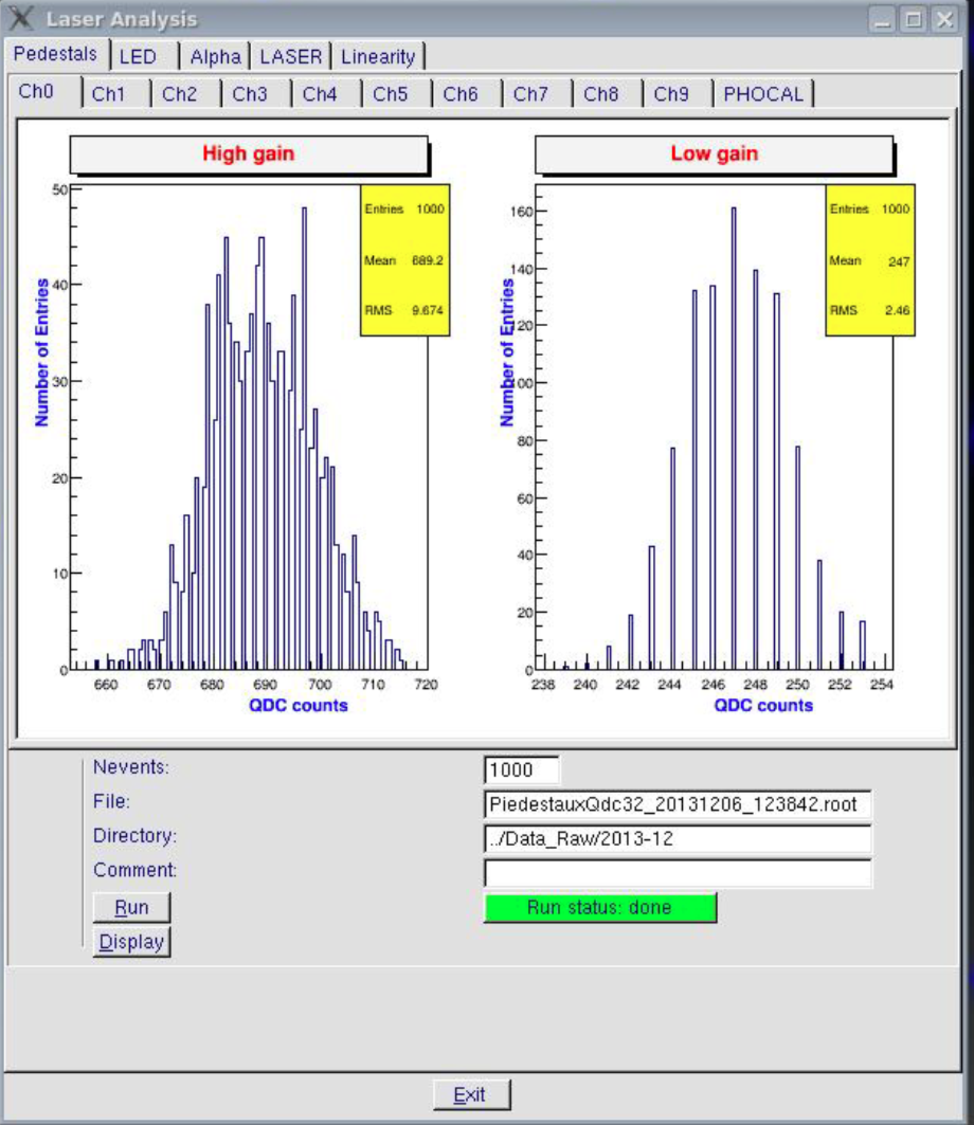
\includegraphics[height=14cm]{figures/Stand_alone_GUI}
\caption{GUI used to run the \lasii~system in the stand-alone mode.}\label{fig:lasstandgui}
\end{figure}

\newpage

%\section{\lasii~data fragments}
%\label{app:b}

\begin{figure}[htbp]
\centering
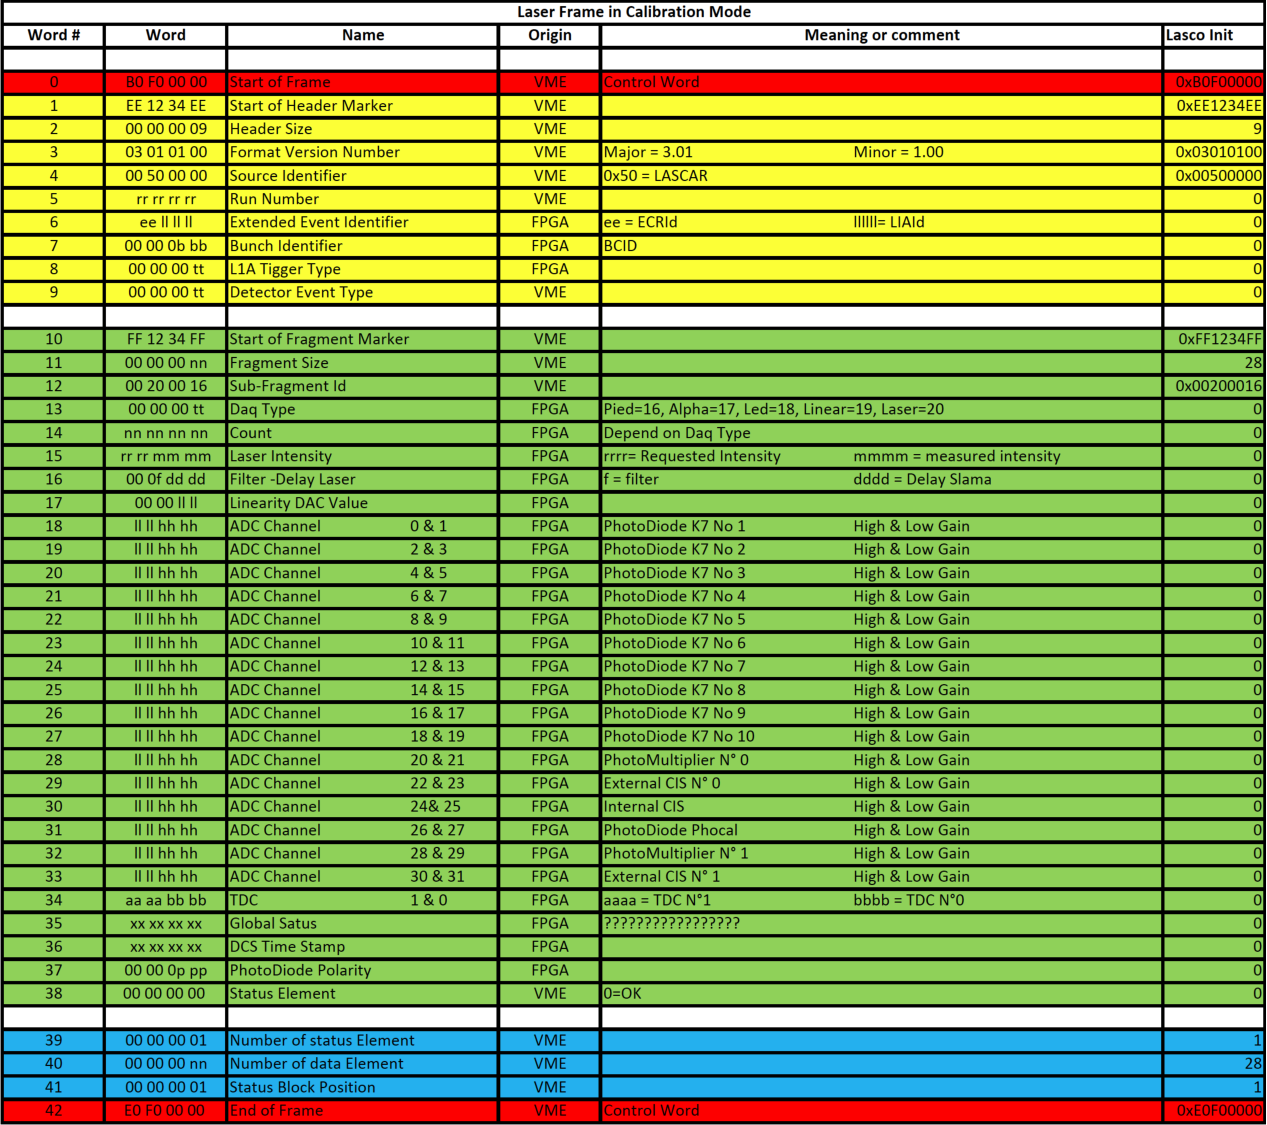
\includegraphics[height=15cm]{figures/short_fragment.pdf}
\caption{Short data fragment structure.}\label{fig:shortfrag}
\end{figure}

\begin{figure}[htbp]
\centering
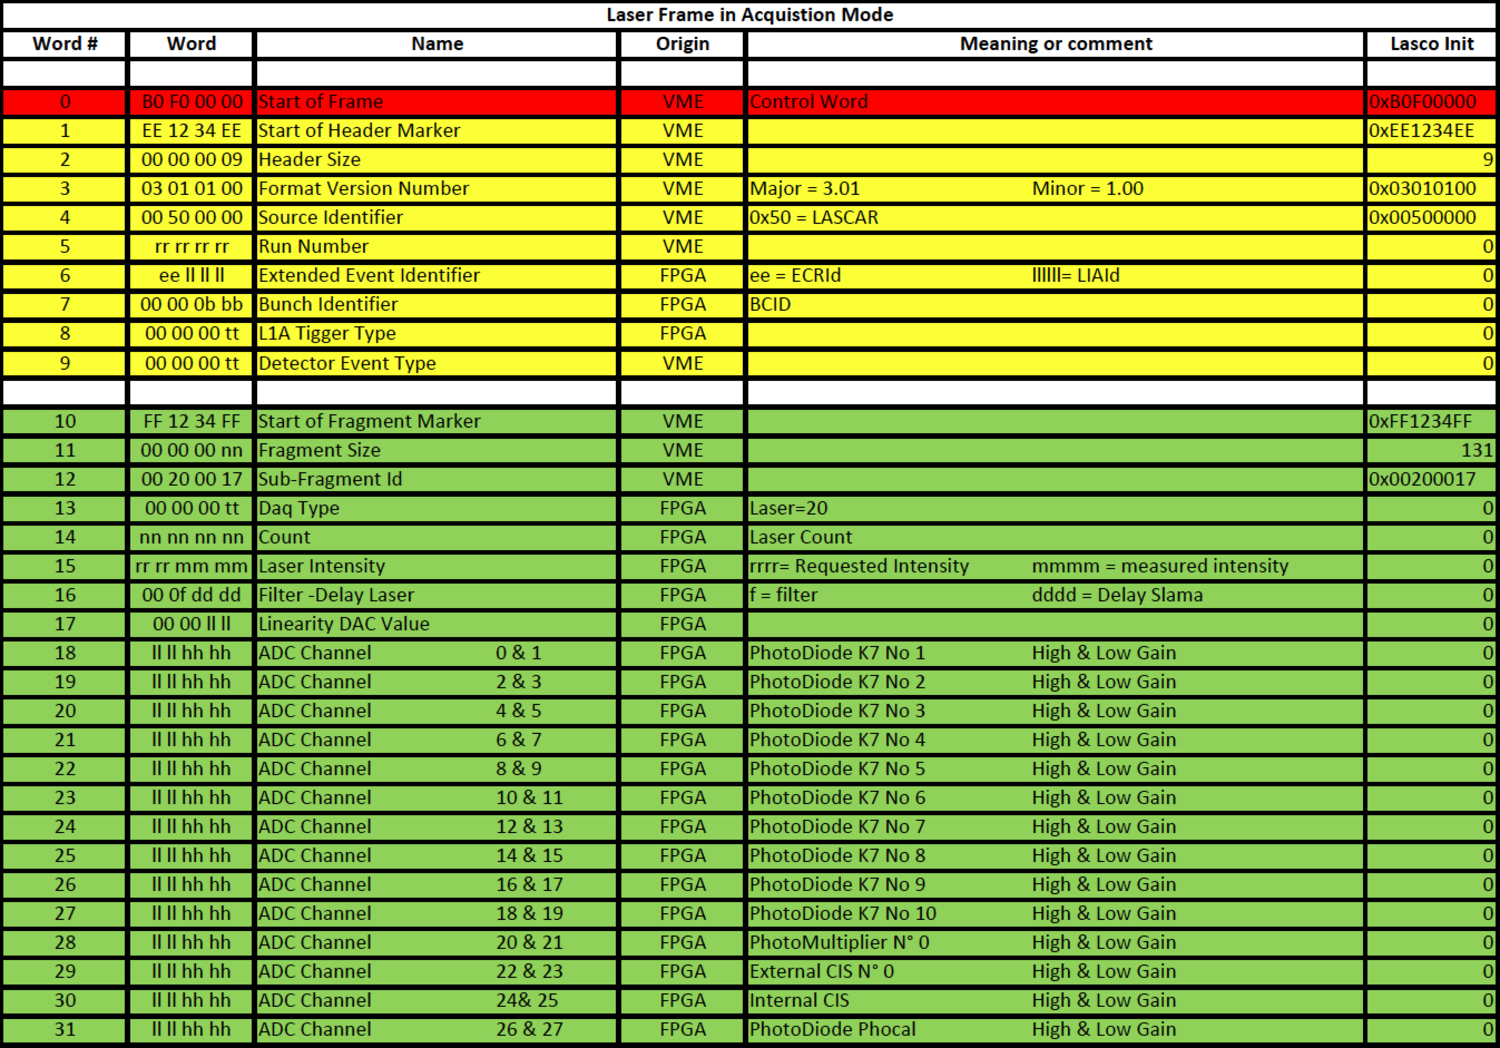
\includegraphics[height=10cm]{figures/long_fragment_1.pdf}
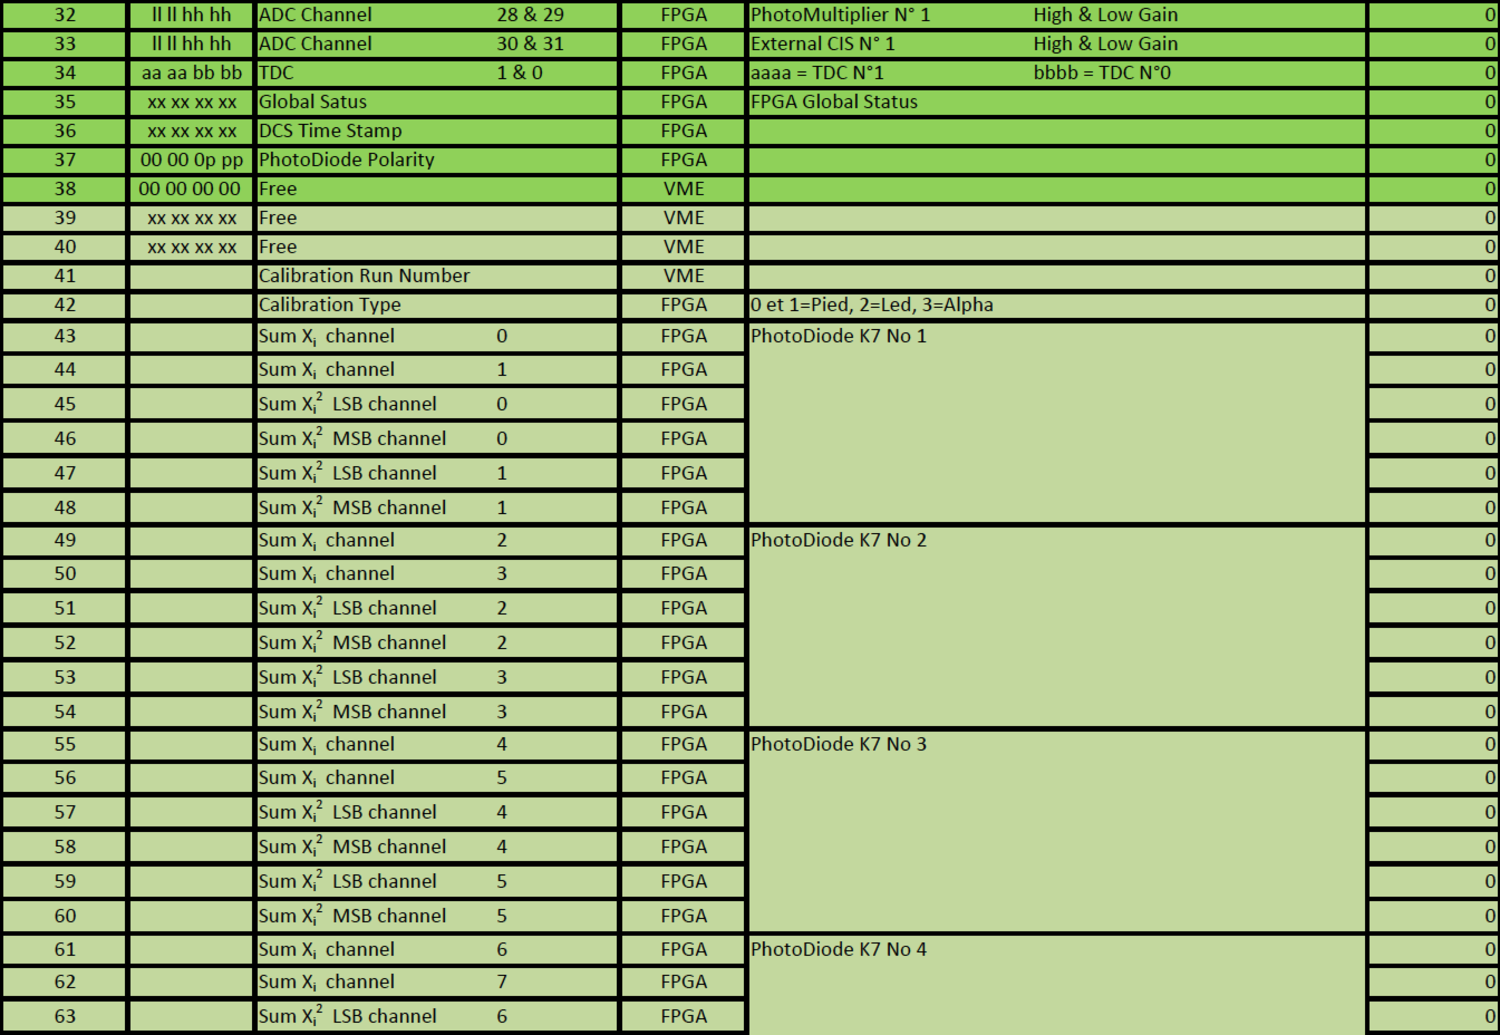
\includegraphics[height=9.9cm]{figures/long_fragment_2.pdf}
\caption{Long data fragment structure.}\label{fig:longfraga}
\end{figure}

\begin{figure}[htbp]
\centering
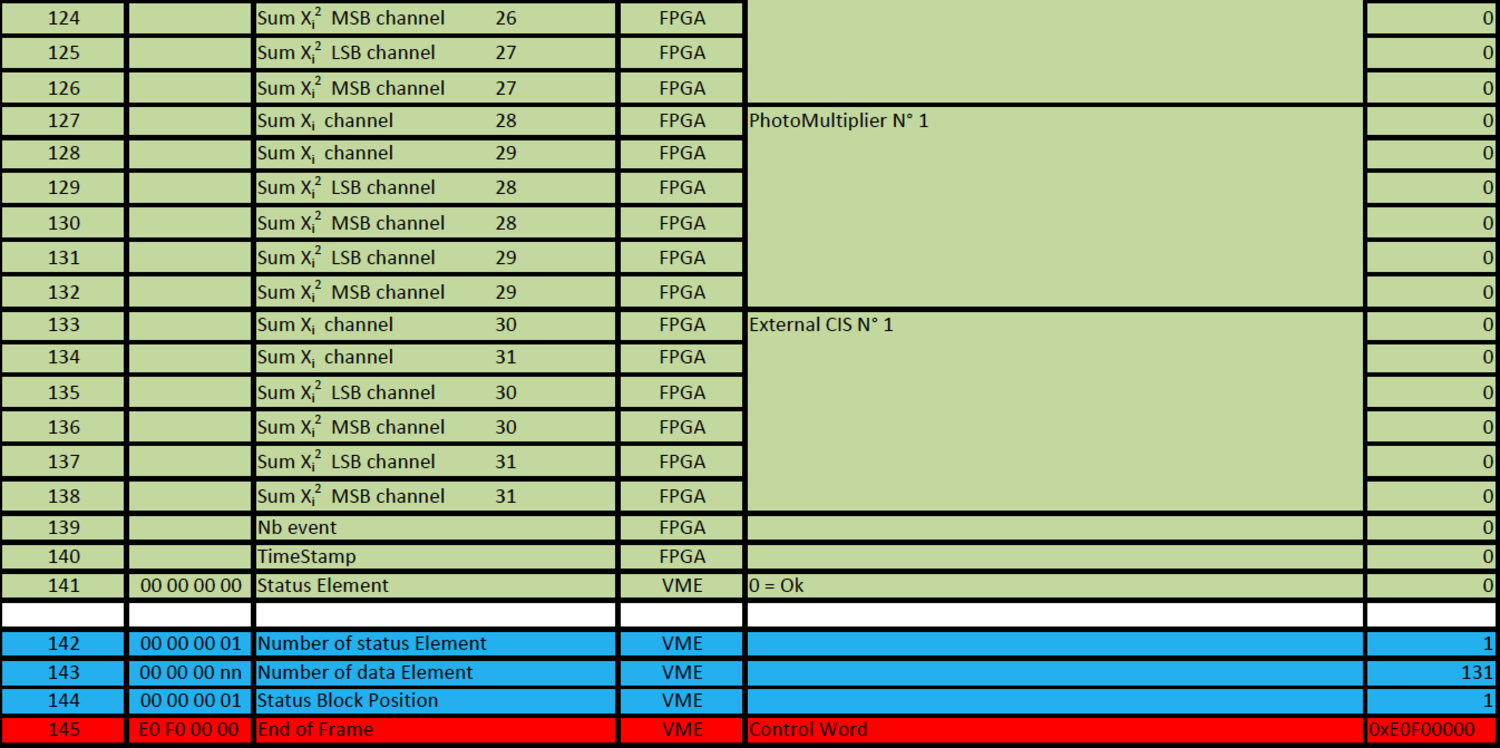
\includegraphics[height=7.5cm]{figures/long_fragment_3.pdf}
\caption{Long data fragment structure (con't).}\label{fig:longfragb}
\end{figure}

\vspace*{5cm}
\newpage

%\section{DAQ parameters published to the IS}
%\label{app:c}

\begin{table}[htbp]
  \begin{center}
\caption{Parameters of the "TileParams.LasIIStatus" object in IS.}\label{tab:IS:lasIIstatus}
{\footnotesize
    \begin{tabular}{lll}
      \hline\hline
      Parameter & Content & Type \\
      \hline
      IsLASCAR & Status of LASCAR & string \\
      DAQmode & LASCAR DAQ mode & string \\
      NbLaserReq & Number of \las{} requests from \shaft{} & u32 \\
      NbLaserReqPump & Number of \las{} requests to the pump & u32 \\
      NbLaserPulses & Number of \las{} pulses emitted by the pump & u32 \\
      NbGates & Number of gates generated by \lascar{} for amplitude digitization & u32 \\
      NbLaserEmit & Number of \las{} emit signals sent to \shaft{} & u32 \\
      NbLaserTT & Number of \las{} Trigger Type received & u32 \\
      NbLaserFrag & Number of \las{} fragments sent & u32 \\
      NbCalibFrag & Number of Calib fragments sent & u32 \\
      NbCISTT & Number of CIS Trigger Type received & u32 \\
      NbCISFrag & Number of CIS fragments sent & u32 \\
      NbOtherTT & Number of other Trigger Type received & u32 \\
      NbDefaultFrag & Number of default fragments sent & u32 \\
      NbL1A & Number of L1A received & u32 \\
      LastEvtID & Last Extended Event ID sent & u32 \\
      LastBCID & Last BCID sent & u32 \\
      LastTT & Last Trigger Type sent & u32 \\
      LastLaserEvtID & Last Extended Event ID sent for a \las{} fragment & u32 \\
      LastLaserBCID & Last BCID sent for a \las{} fragment & u32 \\
      LastCISEvtID & Last Extended Event ID sent for a CIS fragment & u32 \\
      LastCISBCID & Last BCID sent for a CIS fragment & u32 \\
      NbToutTT & Number of timeouts while waiting for TT & u32 \\
      NbToutData & Number of timeouts while waiting for TDC and QDC values & u32 \\
      MaxFIFOBCID & Maximum BCID FIFO occupancy & u32 \\
      MaxFIFOEvID & Maximum EvID FIFO occupancy & u32 \\
      MaxFIFOTT & Maximum TT FIFO occupancy & u32 \\
      IsBusy & True if busy for longer than the limit (5~s) & bool \\
      NbBusy & Number of consecutive busies & u32 \\
      NbBusyMax & Maximum number of consecutive busies observed & u32 \\
      NbTTwhileBusy & Number of TT received while being busy & u32 \\
      TXEnabled & True if output link is enabled & bool \\
      LASCARStatus & Global status register of LASCAR & u32 \\
      LastCombined & Timestamp of last internal calibration run & string \\
      LastAutoStop & Timestamp of last automatic stop by watchdog & string \\
      DiodePolarity & Polarity of the photodiodes & u32 \\
      Filter & Filter wheel position & string \\
      Shutter & Shutter state & string \\
      IpumpReq & Requested \las{} pump intensity & u32 \\
      IpumpMeas & Measured \las{} pump intensity & u32 \\
      Ipump & Measured \las{} pump current & string \\
      Tpump & Measured \las{} pump temperature & string \\
      \hline
    \end{tabular}
   %\caption{Parameters of the "TileParams.LasIIStatus" object in IS.}\label{tab:IS:lasIIstatus}
  \end{center}
}
\end{table}

\newpage

%\section{LICORNE panels (internal DCS of the \lasii~system)}
%\label{app:d}

\begin{figure}[htbp]
\centering
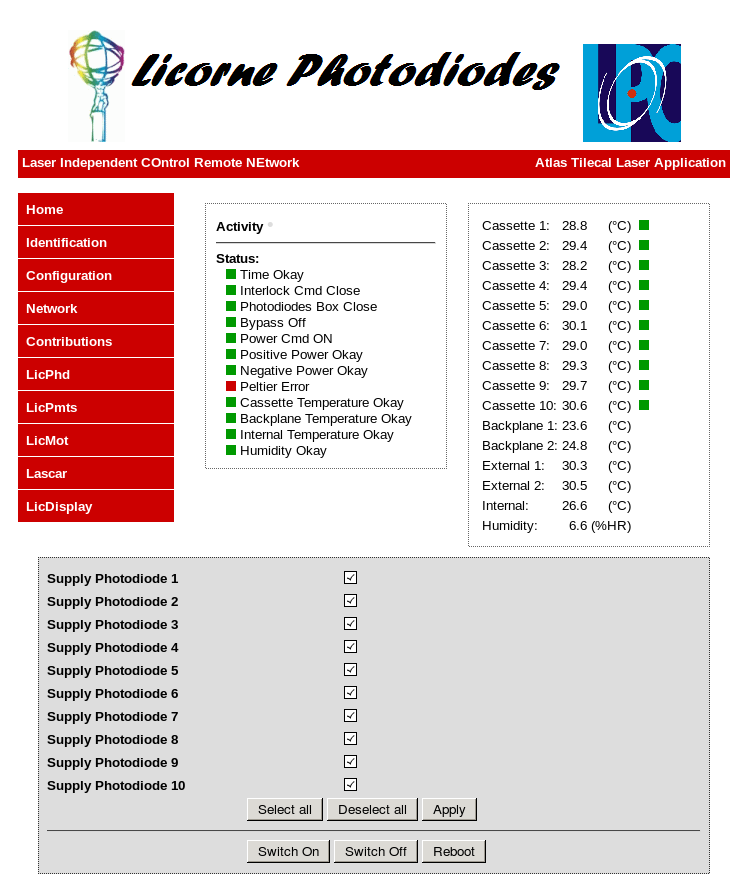
\includegraphics[height=16cm]{figures/licorne_web1.png}
\caption{Web interface view of the internal DCS system : LicPhd panel.}\label{fig:licorne_weba}
\end{figure}

\begin{figure}[htbp]
\centering
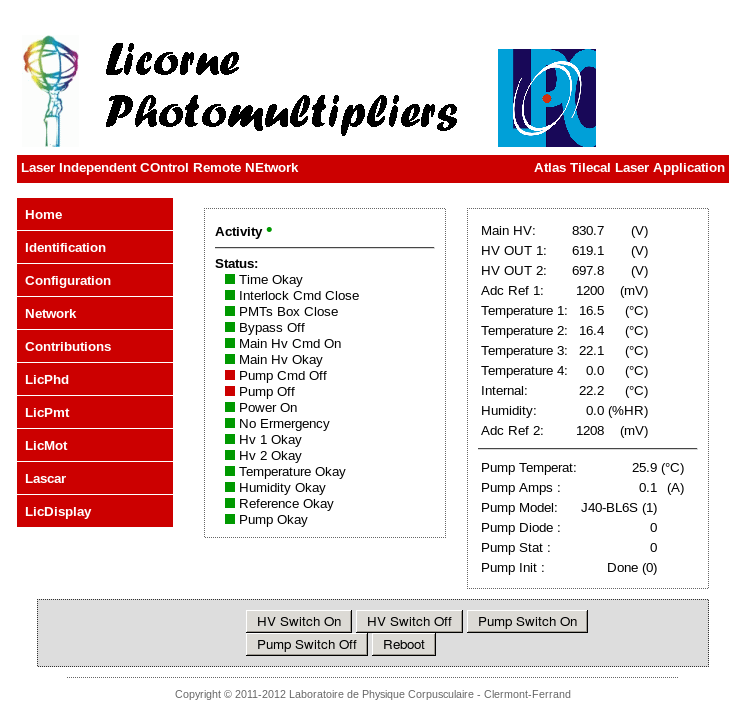
\includegraphics[height=16cm]{figures/licorne_web2.png}
\caption{Web interface view of the internal DCS system : LicPMT panel.}\label{fig:licorne_weba}
\end{figure}


\begin{figure}[htbp]
\centering
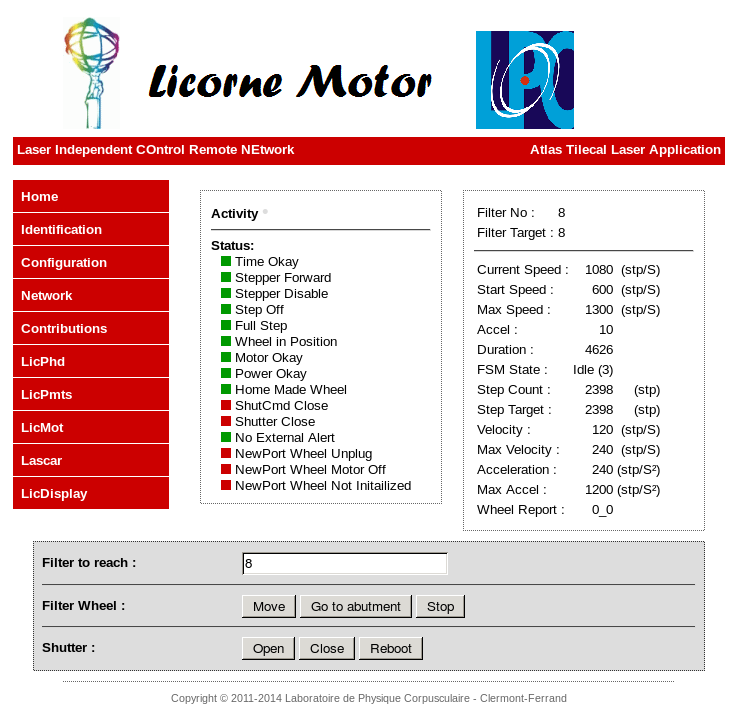
\includegraphics[height=16cm]{figures/licorne_web3.png}
\caption{Web interface view of the internal DCS system : LicMot panel.}\label{fig:licorne_webb}
\end{figure}

\begin{figure}[htbp]
\centering
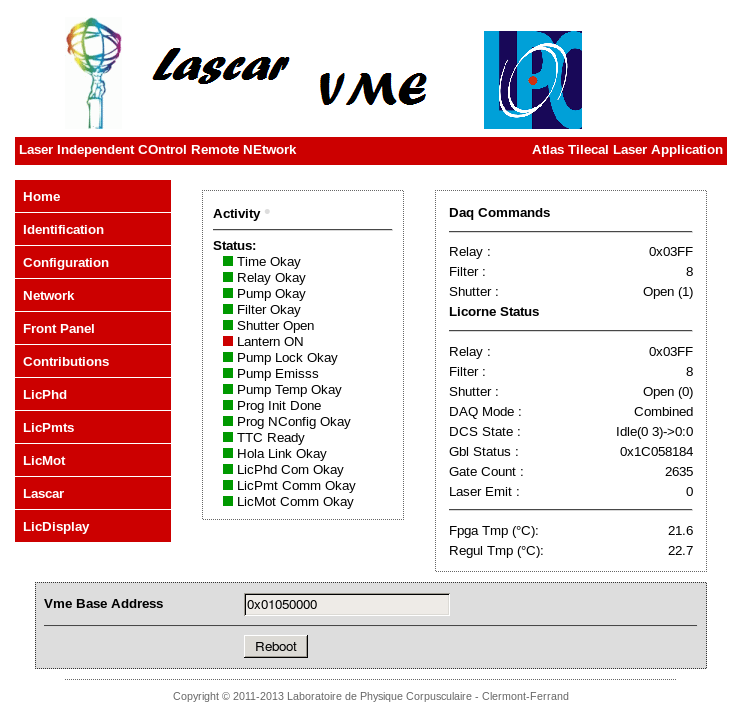
\includegraphics[height=16cm]{figures/licorne_web4.png}
\caption{Web interface view of the internal DCS system :  LASCAR panel.}\label{fig:licorne_webb}
\end{figure}



\newpage

%\section{PVSS DCS panel of the \lasii~system}
%\label{app:e}
\begin{figure}[htbp]
\centering
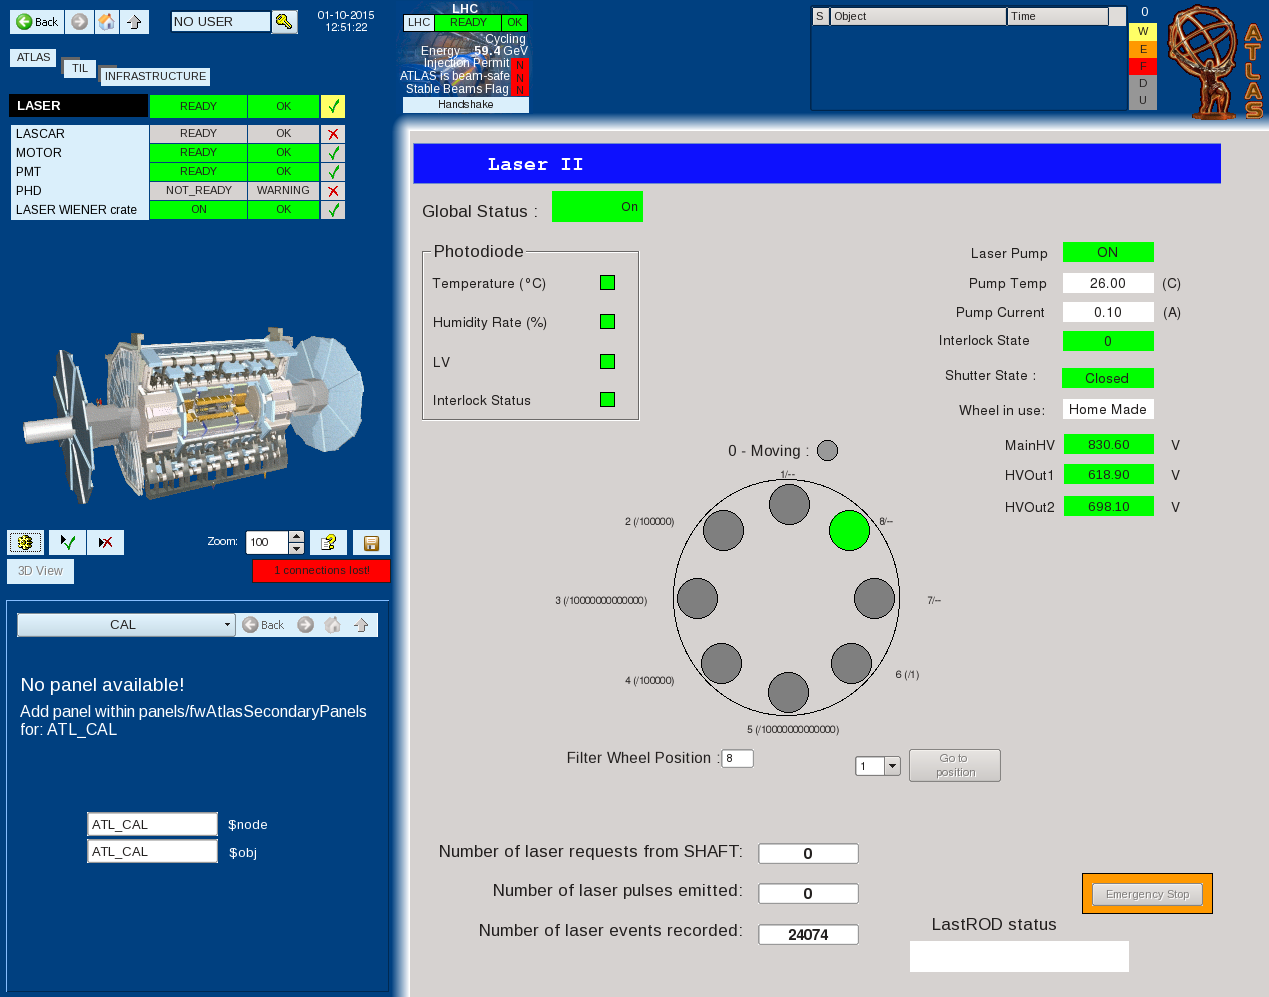
\includegraphics[width=14cm,height=15cm]{figures/dcs_cr_filterwheel.png}
\caption{DCS panel in ATLAS control room : main panel}\label{fig:dcs_cr_a}
\end{figure}

\begin{figure}[htbp]
\centering
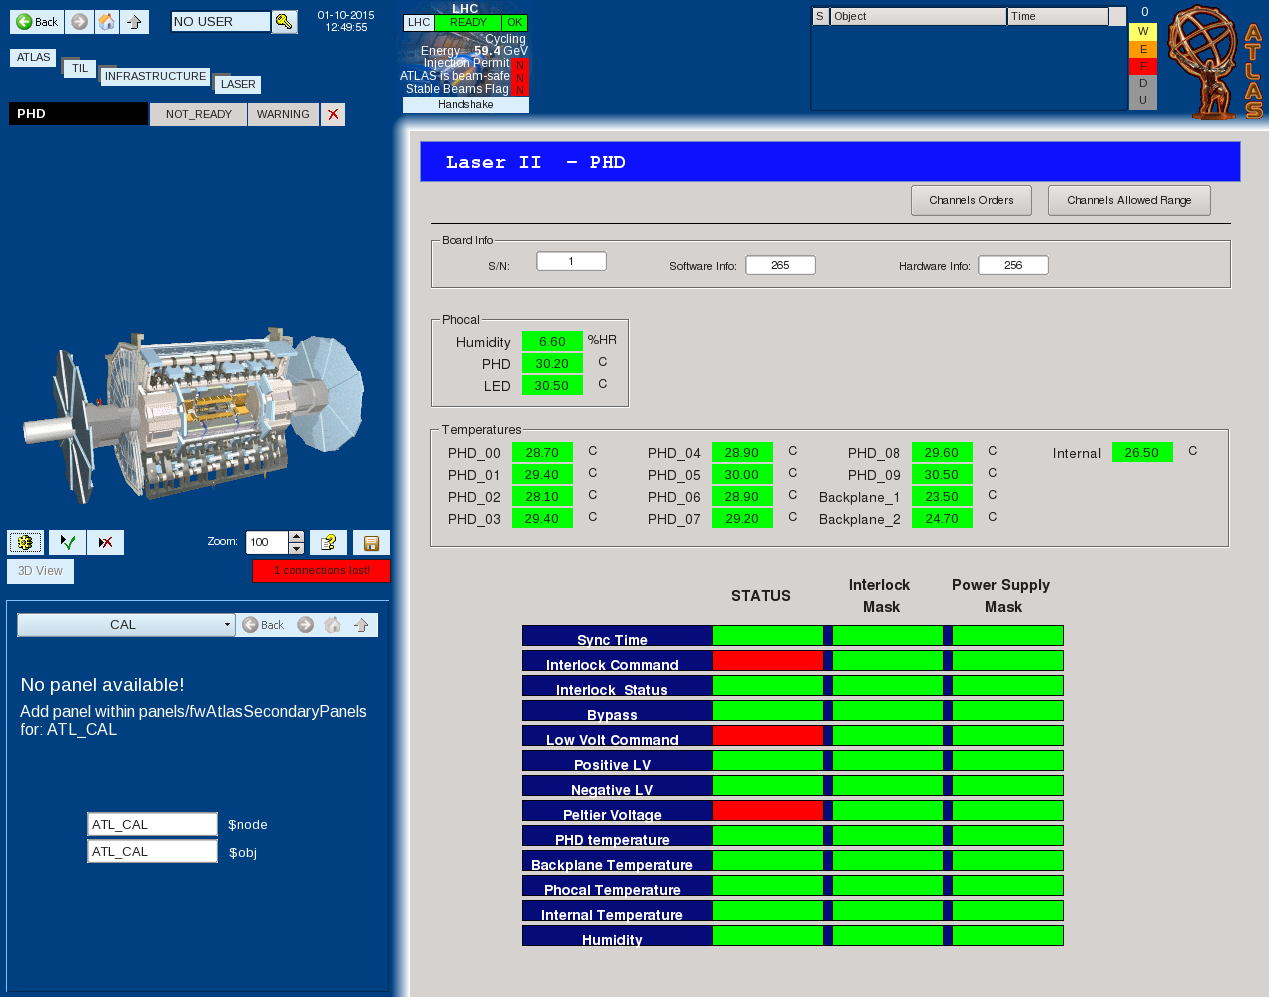
\includegraphics[width=14cm,height=15cm]{figures/dcs_cr_phd.png}
\caption{DCS panel in ATLAS control room : photodiode panel}\label{fig:dcs_cr_b}
\end{figure}

\begin{figure}[htbp]
\centering
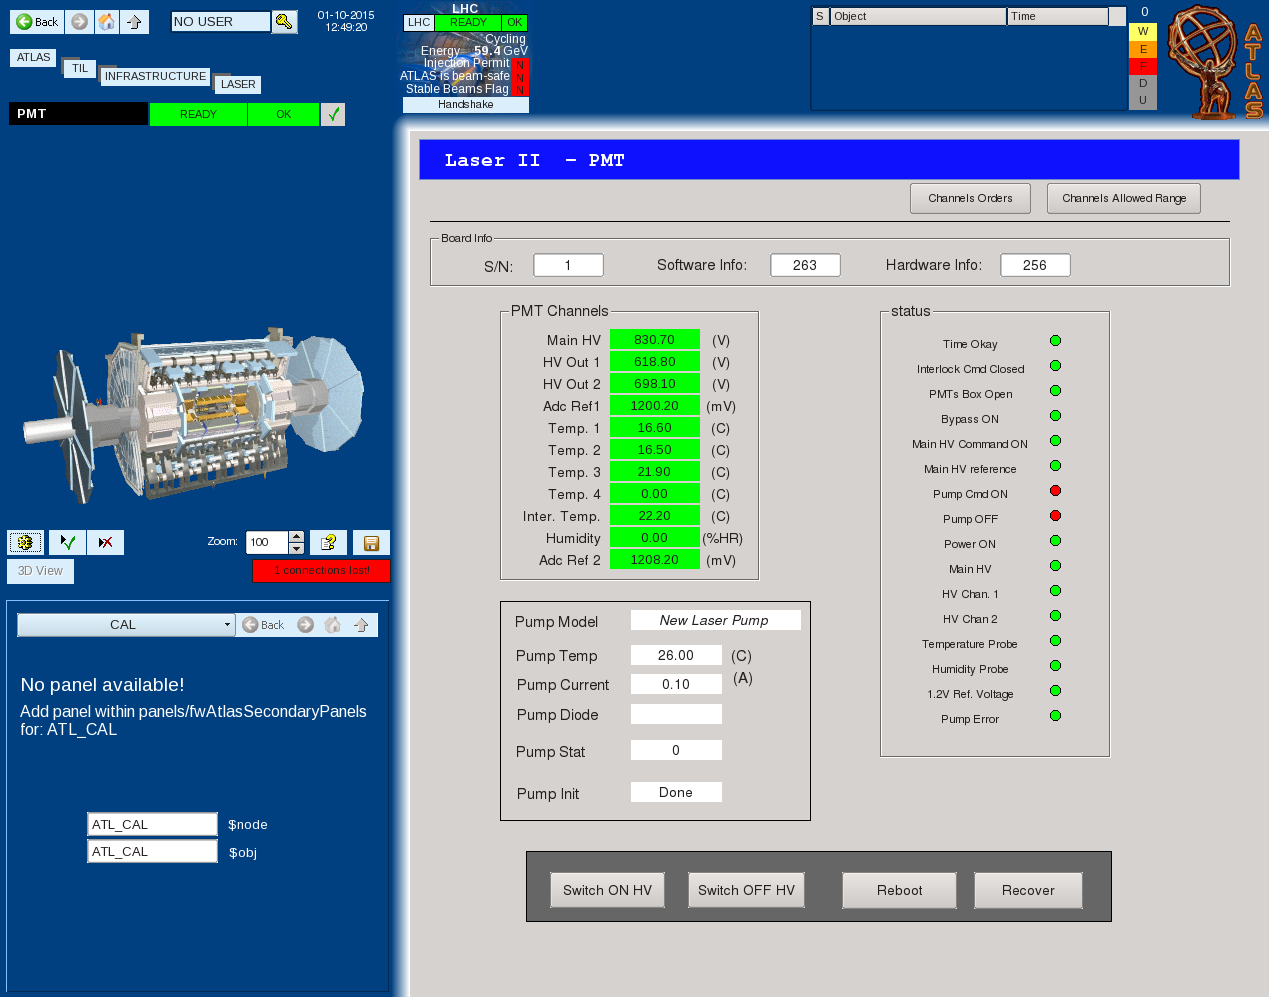
\includegraphics[width=14cm,height=15cm]{figures/dcs_cr_pmt.png}
\caption{DCS panel in ATLAS control room : PMT panel}\label{fig:dcs_cr_c}
\end{figure}

\begin{figure}[htbp]
\centering
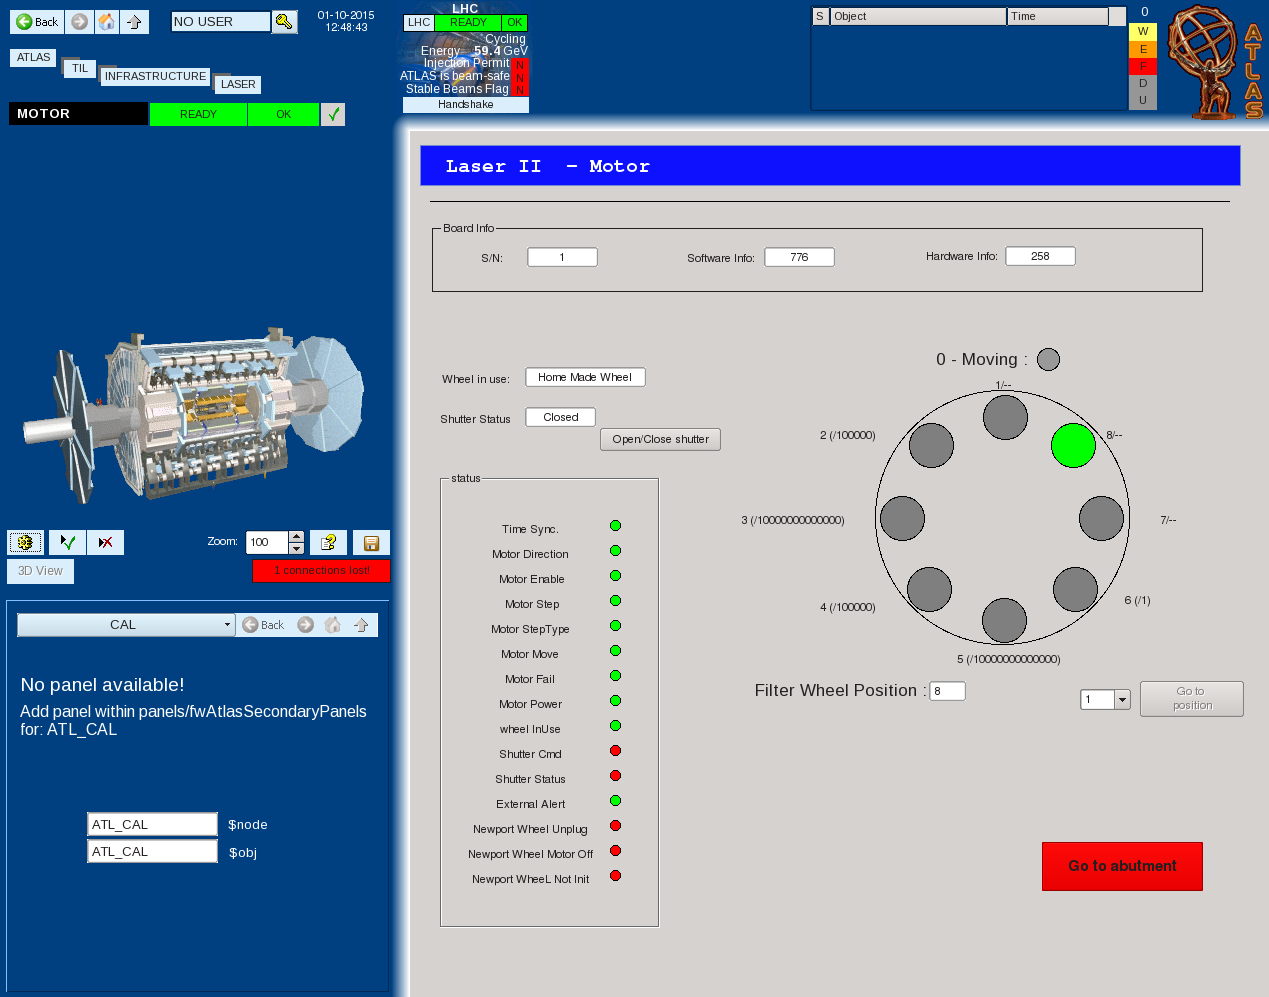
\includegraphics[width=14cm,height=15cm]{figures/dcs_cr_motor.png}
\caption{DCS panel in ATLAS control room : motor panel}\label{fig:dcs_cr_d}
\end{figure}

\begin{figure}[htbp]
\centering
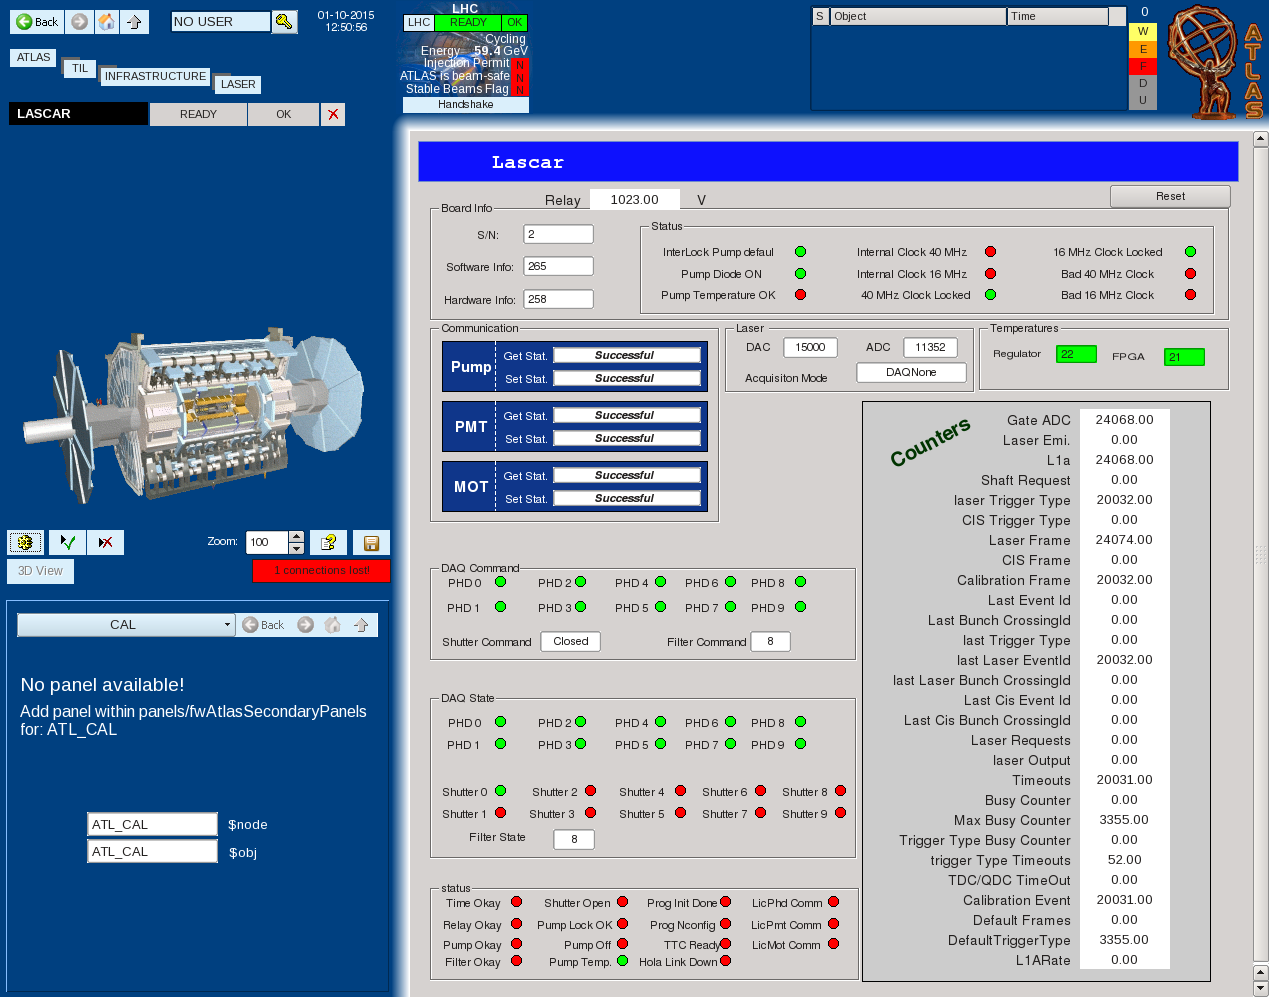
\includegraphics[width=14cm,height=15cm]{figures/dcs_cr_lascar.png}
\caption{DCS panel in ATLAS control room : LASCAR panel}\label{fig:dcs_cr_e}
\end{figure}

\newpage
\end{appendices}